\begingroup
	\pgfdeclarelayer{background layer}
	\pgfsetlayers{background layer,main}
	\tikzstyle{zero}=[circle,draw=black,fill=white,inner sep=0pt,minimum size=2.5mm]
	\tikzstyle{one}=[circle,draw=black,fill=black,inner sep=0pt,minimum size=2.5mm]
		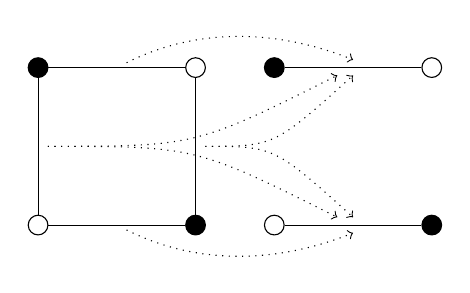
\begin{tikzpicture}
			\node (1) at (-1,-1) [zero] {};
			\node [white] (a) at (1,-1) [one] {};
			\node (0) at (1,1) [zero] {};
			\node [white] (b) at (-1,1) [one] {};
			
			\node (x) at (2,-1) [zero] {};
			\node [white] (y) at (4,-1) [one] {};
			
			\node (w) at (4,1) [zero] {};
			\node [white] (z) at (2,1) [one] {};
			
			\node (psi0) at (0,1) {};
			\node (psi1) at (0,-1) {};
			\node (01a) at (1,0) {};
			\node (01b) at (-1,0) {};
			
			
			\draw (1) -- (a);
			\draw (1) -- (b);
			\draw (a) -- (0);
			\draw (b) -- (0);
			\draw (x) -- (y);
			\draw (w) -- (z);
			
			\draw [->,dotted](psi0) .. controls (1,1.5) and (2,1.5) .. (3,1.1);
			\draw [->,dotted](psi1) .. controls (1,-1.5) and (2,-1.5) .. (3,-1.1);
			\draw [->,dotted](01a) .. controls (2,0) and (2,0) .. (3,-.9);
			\draw [->,dotted](01a) .. controls (2,0) and (2,0) .. (3,.9);
			\draw [->,dotted](01b) .. controls (1,0) and (1,0) .. (2.8,-.9);
			\draw [->,dotted](01b) .. controls (1,0) and (1,0) .. (2.8,.9);
		\end{tikzpicture}		
	%\label{fig:eg_carrier_edges}	
\endgroup